\documentclass[
	12pt, %Schriftgröße
	a4paper, %Papierformat
	oneside, %einseitiger Druck, für zweiseitigen Druck weglassen
%	openany, %neue Kapitel dürfen auch auf linker Seite beginnen (beidseitiger Druck), sonst openright (default)
	chapterprefix, %Kapitelüberschriften zu Beginn eines Kapitels anzeigen
	listof=totoc, %Verzeichnisse (Abbildungen/Tabellen) im Inhaltsverzeichnis aufführen
%	draft, %Entwurfsmodus: lässt Links und Abbildungen weg, zeigt übervolle Zeilen an, wird schneller gesetzt
]{scrbook}

\newcommand*{\universitaet}[1]{\def\universitaet{#1}}
\newcommand*{\fach}[1]{\def\fach{#1}}
\newcommand*{\arbeitsart}[1]{\def\arbeitsart{#1}}
\newcommand*{\titel}[1]{\def\titel{#1}}
\newcommand*{\autor}[1]{\def\autor{#1}}
\newcommand*{\gutachter}[1]{\def\gutachter{#1}}
\newcommand*{\zweitgutachter}[1]{\def\zweitgutachter{#1}}
\newcommand*{\abteilung}[1]{\def\abteilung{#1}}
\newcommand*{\department}[1]{\def\department{#1}}
\newcommand*{\ort}[1]{\def\ort{#1}}
\newcommand*{\datum}[1]{\def\datum{#1}}

%---------------------------------
%---Sprache, Schrift & Encoding---
%---------------------------------

\usepackage[ngerman]{babel} %neue deutsche Rechtschreibung
\usepackage[utf8]{inputenc} %alternativ: ansinew (windows), latin1, latin9 (Linux/UNIX/Mac)

%\usepackage[T1]{fontenc} %einkommentieren, wenn Buchstaben/Schriftbild schief aussehen!
%\usepackage{lmodern} %andere Schrift, sieht evtl. besser aus

%------------
%---Layout---
%------------

\usepackage[
	left=3cm, %linker Seitenrand
	right=3cm, %rechter Seitenrand
	top=2.5cm, %oberer Seitenrand
	bottom=2.5cm, %unterer Seitenrand
]{geometry}
\usepackage[onehalfspacing]{setspace} %1,5-facher Zeilenabstand

%\usepackage{indentfirst} %rückt auch den ersten Absatz eines (Unter)abschnitts ein, so wie alle anderen Absätze auch

\usepackage[
	headsepline, %Kopfzeile durch Querlinie abheben
%	footsepline, %Fußzeile durch Querlinie abheben
	draft=false, %Kopf-/Fußzeile auch im draft-Modus (siehe documentclass) anzeigen
]{scrlayer-scrpage}
\clearpairofpagestyles
\ihead[]{\headmark} %Kapitel-/Abschnittsname innen in der Kopfzeile, außer zu Beginn neuer Kapitel
%\chead[]{}
\ohead*[]{\pagemark} %Seitenzahl außen in der Kopfzeile, außer zu Beginn neuer Kapitel
%\ifoot[]{}
%\cfoot[]{}
\ofoot*[\pagemark]{} %Seitenzahl außen in die Fußzeile, aber nur zu Beginn neuer Kapitel

\renewcommand*\chapterformat{\chapapp~\thechapter} %Kapitelüberschriften in der Form Kapitel~<Nummer>, siehe dazu chapterprefix in der documentclass

%-----------
%---Mathe---
%-----------

\usepackage{amsmath}
\usepackage{amsfonts}
\usepackage{amssymb}

%---------------
%---Sonstiges---
%---------------

\usepackage[sort&compress]{natbib} %ermöglicht die Verwendung von \citet{} und \citep{}
\bibliographystyle{dinat} %Zitierstil: andere auch möglich, z.B. alphadin, plain, ...

\usepackage{caption}
\usepackage{subcaption}
\usepackage{graphicx}
\usepackage{float}

\usepackage{enumerate}

\usepackage[
	textsize=tiny, %kleinere Schrift als die default-Größe in den Notizen, damit mehr reinpasst
]{todonotes} %Notizen im Text mit \todo{<Notiz>} erstellen

%------------------
%---Links & URLs---
%------------------

%hyperref möglichst als letztes package laden (es gibt aber Ausnahmen)!

\usepackage[
	urlcolor=black, %Textfarbe von Links schwarz statt blau (default)
]{hyperref} %für Referenzen, Verweise, Links, ...

%-----------------------------
%---Variablen zum ausfüllen---
%-----------------------------

\universitaet{Carl von Ossietzky Universität Oldenburg}
\fach{Informatik} %Informatik, ...
\arbeitsart{Bachelorarbeit} %Masterarbeit, Diplomarbeit, ...
\titel{Entwicklung einer Augmented Reality Anwendung zum Tracken und Erstellen von Markern für den Bildungsbereich}
\autor{Johannes Scheibe}
\gutachter{Prof. Dr.-Ing. Jürgen Sauer}
\zweitgutachter{M. Sc. B. Eng. Nils Hartmann}
\abteilung{Abteilung Systemanalyse und -optimierung}
\department{Department für Informatik}
\ort{Oldenburg}
\datum{\today} %Tag der Abgabe BEIM PRÜFUNGSAMT

%----------------
%---Titelseite---
%----------------

\begin{document}

\frontmatter %römische Seitennummerierung für den Anfang



\makeatletter
\begin{titlepage}
\centering
\begin{figure}[htb]
  \centering
  \begin{subfigure}{0.5\textwidth}
    \centering
    
\includegraphics[scale=1.8]{Abbildungen/uni_ol_logo.png}
    \end{subfigure}%
    \begin{subfigure}{0.5\textwidth}
      \centering
      
\includegraphics[scale=0.35]{Abbildungen/abteilungslogo.jpg}
    \end{subfigure}
\end{figure}

{\scshape\Large\universitaet\par}
\vspace{1cm}
{\scshape\normalsize\fach\par}
{\scshape\normalsize\arbeitsart\par}

\vfill

\hrule
\vspace{1cm}
{\LARGE\bfseries\titel\par}
\vspace{1cm}
\hrule

\vfill

\begin{minipage}[t]{0.4\textwidth}
  \begin{flushleft}
    {\normalsize\itshape Autor:\par}
    {\normalsize\autor}
  \end{flushleft}
\end{minipage}%
\begin{minipage}[t]{0.4\textwidth}
  \begin{flushright}
    {\normalsize\itshape Erstgutachter:\par}
    {\normalsize\gutachter}
  \end{flushright}
  \begin{flushright}
    {\normalsize\itshape Zweitgutachter:\par}
    {\normalsize\zweitgutachter}
  \end{flushright} 
\end{minipage}

\vfill

{\normalsize\abteilung\par}
{\normalsize\department\par}
\vspace{1cm}
{\normalsize\ort{}, \datum\par}
\end{titlepage}
\makeatother

%---------------
%---Abstracts---
%---------------

%einkommentieren, falls benötigt
%\chapter*{Zusammenfassung}
Auf Deutsch.
%\chapter*{Abstract}
In English.

%-------------------
%---Verzeichnisse---
%-------------------

\tableofcontents %Inhaltsverzeichnis erzeugen
\listoffigures %Abbildungsverzeichnis erzeugen
\listoftables %Tabellenverzeichnis erzeugen

\chapter{Abkürzungsverzeichnis}

\begin{center}
\begin{tabular}{rl}
\textbf{AR} & \textbf{A}ugmented \textbf{R}eality \\ 
\textbf{VR} & \textbf{V}irtual \textbf{R}eality \\ 
\textbf{API} & \textbf{A}pplication \textbf{P}rogramming \textbf{I}nterface \\ 
\textbf{ART} & \textbf{A}ndroid \textbf{R}un\textbf{t}ime \\
\textbf{IDE} & \textbf{I}ntegrated \textbf{D}evelopment \textbf{E}nvironment \\
\textbf{IDE} & \textbf{I}\textbf{d}entifikator \\
\end{tabular}
\end{center}
  %auskommentieren, falls nicht benötigt

%---------------
%---Hauptteil---
%---------------

\mainmatter %arabische Seitennummerierung und nummerierte Kapitel ab dem Hauptteil

%die Kapitel der Arbeit in einzelnen Dateien anlegen und mit \input{} importieren
\chapter{Einleitung}\label{chapter:Einleitung}


\section{Motivation}\label{Motivation}
\section{Ziele der Arbeit}\label{Ziele}
\section{Aufbau der Arbeit}\label{Aufbau}

\chapter{Grundlagen}\label{sec:Grundlagen}


\section{Augmented Reality}\label{AR}
\section{OpenGL}\label{OpenGL}

\chapter{Verwandte Arbeiten}\label{chapter:arbeiten}
In diesem Kapitel werden verwandte Arbeiten betrachtet, die sich mit der Forschungsfrage \glqq Wie lassen sich die Konzepte der Augmented Reality für den Bildungsbereich nutzen?\grqq{} oder einer angrenzenden Thematik beschäftigen. Dabei wird sowohl auf allgemeine Literatur, Studien, wissenschaftliche Arbeiten, als auch konkrete Anwendungen eingegangen und ihr Inhalt zusammengefasst.


\section{Augmented Reality in der Bildung}
Im folgenden werden Veröffentlichungen betrachtet, die sich mit dem Einsatz von Augmented Reality beschäftigen. Zum Teil beleuchteten die Arbeiten konkrete Einsatzmöglichkeiten von Augmented Reality, zum Anderen werden die Vorteile von Augmented Reality oder Richtlinien für AR-Anwendungen betrachtet.


\subsection{Geroimenko: Augmented Reality in Education}
Das Buch \citep{geroimenko:ar-in-education} von \citeauthor{geroimenko:ar-in-education} beschäftigt sich mit dem Einsatz von Augmented Reality im Bildungsbereich. Dabei wird zum einen auf den aktuellen Stand und aktuelle Einsatzbereiche eingegangen, zum Anderen wird aber auch die Konkrete Entwicklung von AR-Anwendungen für den Bildungsbereich thematisiert. Im folgenden werden einmal die Grundaussagen des Buches zusammengefasst:

\subsubsection{Aktueller Stand}
Smartphones stellen aufgrund des Vorhandenseins verschiedener Software Development Kits (SDK) und ihrer Allgegenwart die aktuelle Hauptplattform für Augmented Reality dar. Während Head Mounted Displays vor allem an kleinere Zielgruppen und den professionellen Markt richten. \citep[Kapitel 1.2]{geroimenko:ar-in-education}\\
\begin{figure}
\centering
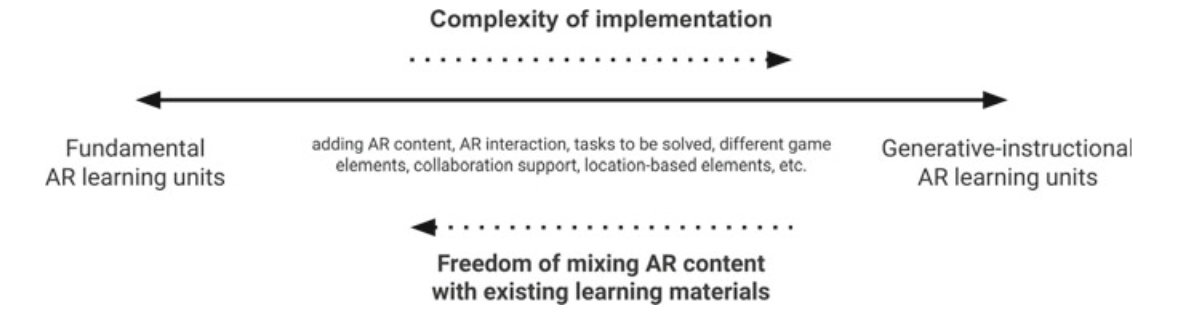
\includegraphics[width=1.0\textwidth]{Abbildungen/ar-object-continuum.png}
\caption[Komplexitätskontinuum von AR-Objekten]{Das Komplexitätskontinuum von AR-Objekten. (Quelle: \cite[S. 9]{geroimenko:ar-in-education})}
\label{fig:komplexitätskontinuum}
\end{figure}
Generell kann bei AR-Objekten zwischen fundamentalen und generativen AR-Lerneinheiten unterschieden werden, die jeweils eine Ende eines Kontinuums darstellen (vergleiche Abbildung \ref{fig:komplexitätskontinuum}).
Der ausschlaggebende Faktor ist dabei die Komplexität des Objektes, je höher diese ist desto generativer ist die Lerneinheit, aber umso geringer ist die Möglichkeit die AR-Inhalte mit den existierenden Lerninhalten zu verbinden. 
Generative AR-Lerneinheiten stehen dementsprechend mehr für sich alleine und decken ein größeres inhaltliches Feld ab.
Der Zugriff auf diese fundamentalen AR-Inhalte ist heutzutage bereits sehr einfach und die Entwicklung in der Thematik wird sich vermutlich ähnlich analog zu der Entwicklung der VR-Inhalte, bei welcher die generative Inhalte nach und nach hinzukamen, verhalten.\citep[Kapitel 1.3]{geroimenko:ar-in-education}\\
Die aktuelle Hauptzielgruppe im schulischen Bereich ist dabei die weiterführende Schule. Außerhalb des schulischen Umfeldes kann AR zur Ausbildung von Fachkräften eingesetzt werden. \citep[Kapitel 1.5]{geroimenko:ar-in-education}

\subsubsection{Entwicklung von Augmented Reality Anwendugen}
Vor der Entwicklung einer Augemented Reality Anwendung für den Bildungsbereich, sollten folgende Entscheidungen getroffen werden:
\begin{enumerate}
\item Die erste Entscheidung, die bei der Entwicklung getroffen werden muss bezieht sich auf die eingesetzte Technologie. Dabei muss überlegt werden, welche Geräte die Schüler bereits besitzen und welche alternativ angeschafft werden können. Des weiteren muss bedacht werden, dass auch die Lehrenden im Umgang mit den neuen Technologie geschult werden müssen.
\item Als zweites muss überlegt werden, was durch den Einsatz der Anwendung erreicht werden soll. Dabei muss grundsätzlich zwischen fundamentalen Lerneinheiten, die angeschaut und vom Nutzer manipuliert werden können, und generativen, instruktiven Lerneinheiten, welche verschiedenen Interaktionsmöglichkeiten, Spielelemente, Beteiligungsformen und vieles mehr enthalten,  abgewogen werden. 
\item Des weiteren muss bedacht werden, dass für die Erstellung von AR-Lernobjekten unter Umständen komplexe Fähigkeiten notwendig sind. Während einfache, dreidimensionale Objekte einfach anhand von Bildern realer Objekte generiert werden können, ist die Erstellung komplexer Lerninhalte aufgrund mangelnder Werkzeuge sehr aufwendig und erfordert weitere Spezialkräfte.
\item Der letzte Punkt ist die Zielgruppe. Hier muss zwischen einem breitem Feld an Einsatzgebieten, wie Schulen, Museen und vielem mehr, abgewogen werden, da sich die Anforderungen der Teilgebiete stark unterscheiden können. 
\end{enumerate}
\citep[Kapitel 1.7]{geroimenko:ar-in-education}

\subsubsection{Augmented Reality in der Lehre}
In der Lehre kann Augemented Reality ein breites Feld bedienen.\\
Ein Einsatzbereich stellen dabei die Naturwissenschaften und die Medizin dar.
Besonders Letzteres kann von Augmented Reality in den folgenden Bereichen profitieren:
\begin{itemize}
\item Anatomie: Hierbei kann AR von Medizinstudenten dazu genutzt werden die Anatomie des Körpers besser zu verstehen, indem sie 3D Modelle im AR-Bereich bertrachten können.
\item Mentoring: Mit Hilfe von AR ist es möglich das Studenten Prozeduren kennenlernen und erfahren, in denen sie noch nicht geschult sind. 
\item Klinische Fertigkeiten: Auch die klinischen Fähigkeiten der Studenten können verbessert werden, indem mit der Hilfe von Augmented Reality klinische Simulationen durchgeführt werden.
\end{itemize}
\citep[Kapitel 7-9]{geroimenko:ar-in-education} \\
Augmented Reality kann zudem für die Umweltbildung im Freien genutzt werden. Dabei bietet AR die Möglichkeit die Komplexität der Umgebung aus verschiedenen Perspektiven zu visualisieren, detaillierte und wissenschaftliche Informationen anzuzeigen oder das \glqq unsichtbare\grqq{} sichtbar zumachen.
Dabei ermöglicht es dem Lernenden eine andere Perspektive auf das Sichtbare, in dem es Parameter, wie die Zeit (Vergangenheit, Zukunft), die Skalierung (mikroskopische Sicht, Vogelperspektive) oder die Wahrnehmbarkeit (Unsichtbares enthüllen, Sichtbares verdecken), verändert. \citep[Kapitel 17]{geroimenko:ar-in-education}\\
Auch in Bereichen der Archäologie kann AR als Forschungsinstrument für die Rekonstruktion und Interpretation eingesetzt werden. \citep[Kapitel 17]{geroimenko:ar-in-education}\\
Ein weiterer Bereich, den Augmented Reality abdecken kann, sind die Geisteswissenschaften.
Hier stellt die Erweiterung der Umgebung basierend auf der aktuellen Position des Nutzers durch AR eine wichtige Einsatzmöglichkeit dar. Dadurch lassen sich beispielsweise Zusatzinformationen zu historischen Gebäuden anzeigen und es ist möglich dem Nutzer einen Eindruck zu vermitteln, wie ein Ort in der Vergangenheit einmal aussah. \citep[Kapitel 11-12]{geroimenko:ar-in-education}\\
Im Bereich des Lernens einer Fremdsprache, bietet AR die Möglichkeit das konventionelle Lernen im Klassenzimmer um eine virtuelle Welt erweitern, um die Motivation der Lernenden zu steigern. \citep[Kapitel 11-12]{geroimenko:ar-in-education}

\subsubsection{Konkrete Anwendungsbeispiele}
Das FeDiNAR-Projekt stellt ein konkretes Anwendungsbeispiel der Augmented Reality zu Ausbildung von Personen dar. Es hat das Ziel, die Fehler mit Hilfe von Augmented Reality zu einer Lernmöglichkeit umzuwandeln. Das Konzept beruht darauf Fehler nicht durch den Ausbilder zu verhindern, sondern sie zuzulassen. Dieses soll den Ausbilder möglich sein, indem die Auszubildenden zwar an echten Maschinen arbeiten, die Auswirkungen ihrer Handlungen dabei jedoch lediglich in der Augmented Reality dargestellt werden. 
\citep[Kapitel 5]{geroimenko:ar-in-education}\\
Ein weiteres Anwendungsbeispiel ist die im Rahmen des Buches beschriebene Entwicklung einer Online-Plattform zur verbesserten Lernerfahrung. Die Anwendung beruht auf \glqq durchsichtige\grqq{} Markern, die in ein Bild eingefügt werden konnten. Wurde der Marker innerhalb eines Bildes erkannt wird ein dreidimensionales Modell des Bildes mit Hilfe von Augmented Reality angezeigt. \citep[Kapitel 3]{geroimenko:ar-in-education}

\subsection{Hedberg: A Systematic Review of Learning through Mobile Augmented Reality}
In der wissenschaftlichen Arbeit von \citeauthor{hedberg:review-ar-learning} \citep{hedberg:review-ar-learning} wurde mit Hilfe einer systematischen Literaturauswertung eine Einschätzung des Einsatzes von Augmented Reality zu Bildungszwecken vorgenommen. \\
Dabei wurde die Relevanz einzelner Einsatzgebiete anhand der Anzahl an Veröffentlichungen zum jeweiligen Thema gemessen.\\ Die Veröffenntlichungen stammen dabei aus den Datenbanken \glqq IEEE Xplore\grqq , \glqq Elsevier\grqq{} und der \glqq ACM digital libary\grqq{} und wurden über Schlüsselwörter herausgesucht. Die Ergebnisse der Suche wurden im Anschluss noch gefiltert und kategorisiert, um irrelevante Veröffentlichungen auszuschließen.
Anhand der gesammelten wissenschaftlichen Arbeiten kam die Studie zu den folgenden Ergebnissen in den für diese Arbeit relevanten Kategorien:

\subsubsection{Bildungsniveau}
Diese Kategorie zielte darauf ab die Zielgruppen der AR-Systeme herauszufinden. Dabei kam die Studie zu dem Ergebnis, dass die meisten Systeme (fast 50 \%) bezogen auf das amerikanische Bildungssystem für die Universität geschaffen wurden. Mit einem deutlichen Abstand folgt die Grundschule, die Junior High School, die High School und die Vorschule. \citep[S. 78]{hedberg:review-ar-learning}

\subsubsection{Mobiles Endgerät}
In dieser Kategorie ging es darum herauszufinden, welches die meist genutzten Endgeräte für Augmented Reality im Bildungsbereich darstellen. Hierbei kam heraus, dass das Handy bzw. das Smartphone (43,84 \%) gefolgt von dem Tablet (27,40 \%) diese Kategorie dominieren, wobei ebenfalls 27 \% der wissenschaftlichen Arbeiten keine spezifische Plattform angaben. \citep[S. 80]{hedberg:review-ar-learning}

\subsubsection{Unterrichtsfach}
Diese Kategorie untersuchte die fachliche Ausrichtung der Augmented Reality und kam zu dem Ergebnis das die Systeme vor allem in den Naturwissenschaften genutzt werden. Darauf folgen mit signifikantem Abstand die Sprachen, Geschichte und Technik. \citep[S. 81]{hedberg:review-ar-learning}

\subsubsection{Lernerfolge}
Hier bei wurden Studien untersucht, die sich mit dem pädagogischen Nutzen von Augmented Reality beschäftigt haben. Dabei kamen von 73 Studien lediglich zwei nicht zu dem Ergebnis, dass AR einen positiven Einfluss auf das Lernen besitzt.\\
Allgemein stellten 45 Veröffentlichungen (54,88 \%) eine erhöhte Motivation und ein verbessertes Engagement fest. 28 Studien (34,15 \%)konnten verbesserte Lernergebnisse bei den Studenten aufzeigen.  \citep[S. 81-82]{hedberg:review-ar-learning}

\subsubsection{Pädagogische Methoden}
In der letzten Kategorie, wurden die Einsatzarten von Augmented Reality im Bildungsbereich untersucht und das Ergebnis erarbeitet, dass die drei Hauptanwendungsmethoden das interaktive, das forschungsbasierte und das kollaborative Lernen sind. \citep[S. 82]{hedberg:review-ar-learning}


\subsection{Billinghurst: Augmented Reality in Education}\label{sec:billinghurst-ar-education}
\citeauthor{billinghurst:ar-in-education} untersuchte in seiner wissenschaftlichen Arbeit \citep{billinghurst:ar-in-education} den Einsatz von Augmented Reality im Bildungsbereich.\\
Dabei geht er in den folgenden drei Unterkapiteln auf unterschiedliche Eigenschaften der AR im Bildungsbereich ein.

\subsubsection{Nahtlose Interaktion}
\citeauthor{billinghurst:ar-in-education} führt hier auf, dass Schüler besser zusammenarbeiten, wenn sie sich gemeinsam auf einen Arbeitsplatz fokussieren. Dieses ist bei computerbasierten Lernen schwierig um zusetzten, da sich jeder auf den Bildschirm vor sich fokussiert. Dadurch fehlt eine wichtige Eigenschaft, die die Kommunikation in der Gruppe verbessert: die gegenseitige Sichtbarkeit. Wenn Schüler gleichzeitig das Objekt der Diskussion und ihre Diskussionspartnern sehen, werden auch die nichtverbalen Gesprächsmerkmale, wie Gesten oder die Mimik wahrgenommen. Diese Merkmale bilden einen essentiellen Teil der menschlichen Kommunikation. 
Durch den Einsatz von Augmented Reality können diese Eigenschaften bei behalten werden und trotzdem gleichzeitig computerbasierte Inhalte angezeigt werden. \citep[S. 2-3]{billinghurst:ar-in-education}

\subsubsection{Greifbare Schnittstelle}
Hier führt \citeauthor{billinghurst:ar-in-education} auf, dass im Bildungsbereich physische Objekte dazu genutzt werden Bedeutung von theoretischem Wissen zu übermitteln, in dem sie die Eindrücke des Schülers, durch ihre Erscheinung, ihre physkalischen Eigenschaften, ihren räumlichen Beziehungen und der Fähigkeit, die Aufmerksamkeit zu fokussieren, verstärken.\\
Diese Eigenschaften lassen sich zu großen Teilen auch auf die virtuellen Objekte in der Augmented Reality beziehen. Auf Grund der direkten Beziehungen zwischen der virtuellen Objekten und der Augmented Reality ist zum Beispiel eine physikalisch basierte Interaktion mit den computergenerierten Objekten möglich. \citep[S. 3]{billinghurst:ar-in-education}

\subsubsection{Übergangsschnittstelle}
Im dritten Abschnitt bezieht sich \citeauthor{billinghurst:ar-in-education} auf das bereits in Kapitel \ref{sec:ar} eingeführte RV-Kontinuum und führt an, dass man mittels AR den Nutzer entlang des Kontinuums in die virtuelle Welt führen kann. Besonders Kinder können so in die Seiten eines Buches eintauchen und die Fantasie Realität werden lassen. Dadurch werden aus statischen Unterrichtsbüchern dynamische interaktive Umgebungen. \citep[S. 3-4]{billinghurst:ar-in-education}


\subsection{Diegmann: Benefits of Augmented Reality in Educational Environments}\label{sec:diegmann-benefits-ar}
In dem Artikel \citep{diegmann:benefits-ar} von \citeauthor{diegmann:benefits-ar} werden die Vorteile von Augmented Reality betrachtet. \\
Dabei wurde eine systematische Evaluation von Augmented Reality anhand der Veröffentlichungen zu diesem Thema durchgeführt. \\
Basierend auf der Literatur stellte der Artikel zunächst in den folgenden Bereichen positive Effekte der Augmented Reality fest:

\subsubsection{Geisteszustand}
In verschiedenen Veröffentlichungen wurde eine Verbesserung der Motivation festgestellt. Dieses umfasst ein erhöhtes Engagement und Interesse gegenüber den Lerninhalten und der Technologie.\\
Des weiteren wurde auch eine Steigerung der Aufmerksamkeit und der Konzentration, bezogen auf die Inhalte mit denen die Lernenden konfrontiert wurden, festgestellt.\\
Zu dem verbesserte sich auch die Zufriedenheit der Schüler bezüglich der Bildungsfortschritte und des Lernprozesses. 
\citep[Kapitel 4.1]{diegmann:benefits-ar}

\subsubsection{Lehrkonzept}
Das Lehrkonzept verbessert sich durch AR  dahingehend, dass ein schülerzentriertes Lernen ermöglicht, wodurch das unabhängige, eigenverantwortliche Lernen der Schüler, sowie die Fähigkeit Wissensinhalte aufzunehmen verbessert wird.\\
Auch eine Verbesserung des kollaborativen Lernens kann durch AR erreicht werden. Dabei kann Schülern durch AR die Möglichkeit zur gemeinsamen Problemlösung und Kommunikation gegeben werden.
\citep[Kapitel 4.2]{diegmann:benefits-ar}

\subsubsection{Darstellung}
Auch die Darstellung von Lerninhalten kann mit Hilfe von AR-Anwendungen verbessert werden. So können AR-Inhalte einen höheren Detailgrad ermöglichen und die Zugänglichkeit von Lerninhalten und die Interaktivität mit diesen Inhalten. verbessern. Besonders die neuen Interaktionsmöglichkeiten unterstützen ein Lernen durch eigene Erfahrungen.
\citep[Kapitel 4.3]{diegmann:benefits-ar}

\subsubsection{Lerntyp}
Ein weiterer Vorteil ist die Verbesserung der Lernkurve dar. Schüler die mit Hilfe von Augmented Reality Unterrichtsinhalte erfassen konnten lernten schneller und einfacher als Schüler ohne diese Möglichkeit.\\
Auch eine Verbesserung der Kreativität, der Wissensaufnahme und der Problemlösung konnte in verschiedenen Veröffentlichungen festgestellt werden.
\citep[Kapitel 4.4]{diegmann:benefits-ar}

\subsubsection{Verständnis}
Dieser Bereich bezieht sich auf das Wissen, das durch Augmented Reality erlangt werden kann.\\
Dabei kann, neben einem deutlich gesteigertem, räumlichen Verständnisses, auch eine Steigerung des Gedächtnisses beobachtet werden. So konnten Schüler mit Hilfe von AR sich besser an Inhalte erinnern. \\
\citep[Kapitel 4.5]{diegmann:benefits-ar}

\subsubsection{Zuordnung der Vorteile zu verschiedenen Anwendungsarten}
Diese Vorteile lassen sich auf Basis der Literatur zu den folgenden Anwendungsarten zuordnen:
\begin{itemize}
\item Entdeckungsbasiertes Lernen: Bei entdeckungsbasierten Anwendungen erhält der Benutzer \glqq Informationen über einen realen Ort, während er gleichzeitig das interessierende Objekt betrachtet\grqq{} \citep[Kapitel 2.2]{diegmann:benefits-ar} \\
Bei Art von Anwendungen konnte vor allem eine Verbesserung der Lernkurve und des Geisteszustandes bei den Lernenden beobachtet werden. Insgesamt deckt diese Kategorie die meisten Vorteile im Vergleich zu den anderen Anwendungsarten ab. \citep[Kapitel 5]{diegmann:benefits-ar}
\item Objektmodellierung: Diese Gruppe beschreibt Modellierungsanwendungen, die mit Hilfe von Augmented Reality dem Nutzer direktes Feedback zur Optik der modellierten Objekte geben. \citep[Kapitel 2.2]{diegmann:benefits-ar} \\
Bei dieser Anwendungsart konnte in der Literatur eine erhöhte Motivation, eine verbesserte Zufriedenheit und eine angestiegene Lernkurve bei den Studierenden festgestellt werden. Jedoch konnte trotz der starken Interaktion mit der Augmented Reality, keine Artikel gefunden werden die von einer verbesserten Interaktivität oder Kreativität berichteten. \citep[Kapitel 5]{diegmann:benefits-ar}
\item AR-Bücher: AR-Bücher bezeichnen Bücher, die durch Augmented Reality angereichert werden. Dabei stellen sie dem Leser 3D-Darstellungen der Lerninhalte zur Verfügung, wenn dieser das Buch mit Hilfe von speziellen, AR-fähigen Geräten betrachtet. \citep[Kapitel 2.2]{diegmann:benefits-ar}\\
Die wenigsten Veröffentlichungen konnten diese Kategorie abdecken und dem entsprechend wenig Vorteile wurden in den Arbeiten herausgestellt. Lediglich sechs der zuvor definierten Vorteil waren in der Literatur wieder zu finden. \citep[Kapitel 5]{diegmann:benefits-ar}
\item Fähigkeitentraining: Diese Kategorie umfasst Anwendungen die das Trainieren spezieller Fähigkeiten trainieren, in dem sie die Abläufe, Trainingsobjekte oder Ähnliches bereitstellen. \citep[Kapitel 2.2]{diegmann:benefits-ar} \\
Anwendungen die in den Bereich des Fähigkeitentrainings fallen haben in der Literatur die meisten Erwähnungen eines verbesserten Verständnisses. Des weiteren wird häufig eine Verbesserung der Lernkurve erwähnt. \citep[Kapitel 5]{diegmann:benefits-ar}
\item AR-Spiele: In dieser Gruppe befinden sich Video-Spiele, die mit Hilfe von Augmented Reality dem Schüler Lerninhalte vermitteln sollen \citep[Kapitel 2.2]{diegmann:benefits-ar}.
Die Vorteile von AR-Spielen liegen laut der Literatur vor allem im Bereich Bereich des Geisteszustands, der Lernkurve und der Zugänglichkeit zu den Lerninhalten \citep[Kapitel 5]{diegmann:benefits-ar}.
\end{itemize}

\subsection{Dey: A Systematic Review of 10 Years of Augmented Reality Usability Studies}
In dem Artikel \citep{dey:review-of-ar-studies} von \citeauthor{dey:review-of-ar-studies} wird eine Auswertung von verschiedenen Studien, die sich mit dem Einsatz von Augmented Reality beschäftigen, durchgeführt. Dabei wird ein Überblick über die Veröffentlichungen aus den Jahren von 2005 bis 2014 gegeben.\\
Insgesamt wurden in dem Artikel die folgenden Ergebnisse herausgestellt.

\subsubsection{Display}
Allgemein betrachtet stellen Head Mounted Displays (HMD, deutsch: \glqq Am Kopf befestigter Bildschirm\grqq ) und Hand-Held Displays (HHD, deutsch: \glqq Handdisplay\grqq ) die meistgenutzten Wiedergabegeräte dar.\\
Im Bildungsbereich kommen HMDs hingegen kaum zum Einsatz. Hier dominieren vor allem HHDs, gefolgt von Desktopbildschirmen und  verschiedene Arten von großformatigen Anzeigen. \citep[Kapitel 3.7]{dey:review-of-ar-studies}

\subsubsection{Bildungsbereich}
Alle Studien die sich mit dem Einsatz im Bildungsbereich beschäftigten, bezogen sich auf eine Methode des Unterrichtens oder des Lernens. Basierend auf den Schlüsselwörtern der Studien sind vor allem das Lernen, die Interaktivität, die Nutzer und die Umgebung relevant für den Bildungsbereich.\\
Eine Studie von Fonseca u. a, die im Rahmen des Artikels genauer betrachtet wurde, untersuchte den Einsatz einer Smartphone basierten AR-Anwendung, die zur Visualisierung von 3D-Modellen genutzt werden kann, in einem schulischen Umfeld. Dabei beobachteten sie eine erhöhte Motivation und eine Verbesserung der akademischen Leistungen. \\
Diese Anwendung stellt nur ein Beispiel der untersuchten Einsatzmethoden von AR dar. Insgesamt wurden in den Studien die verschiedensten Einsatzmöglichkeiten von Anwendungen untersucht. Darunter waren beispielsweise Applikationen, die Personen mit Amputationen im Umgang mit Prothesen schulen, Anwendungen, die kognitiv beeinträchtigte Menschen bei der Erwerbung von beruflichen Fähigkeiten unterstützen oder AR-Systemen, welche zum Unterrichten der historischen Seiten einer Stadt genutzt werden können. \\
Auf dieser Grundlage betonen die Autoren, die Variabilität in den Einsatzmethoden, die im Bildungsbereich genutzt werden können. \citep[Kapitel 4.2]{dey:review-of-ar-studies}


\subsection{Damberger: Augmented Reality als Bildungsenhancement?}
In dem Artikel \citep{damberger:ar-bildungsenhancement} von \citeauthor{damberger:ar-bildungsenhancement} wird die Frage thematisiert, ob Augmented Reality die Bildungsprozesse verbessern kann. Eine solche Verbesserung, die auf dem Einsatz von Technologien beruht, bezeichnet der Autor als Bildungsenhancement. \\
Dabei wird jedoch betont, dass mit dem Bergriff nicht die Verbesserung der Bildung selbst gemeint ist. Dieses ist mit Hilfe von AR ebenso wenig möglich, wie durch einen gesteigerten Konsum an (Fach-)Literatur, so der Autor.
\begin{quote}
\glqq Bildungsenhancement soll vielmehr einen durch Technik ermöglichten besonderen Zugang zur Welt beschreiben, der reflexive Prozesse eröffnet, in deren Folge ein Mehr an Bildung möglich werden kann.\grqq \citep[S. 5]{damberger:ar-bildungsenhancement}
\end{quote}
Im Laufe des Artikels betrachtet der Autor, die oben genannte Frage aus einer philosophischen Sicht.

\subsubsection{Augmented Reality als Erweiterung der Realität}
Augmented Reality bietet dem Menschen die Möglichkeit seine Umgebung mit virtuellen Objekten zu ergänzen. Dieses Fähigkeit bietet großes didaktisches Potential, indem sie es dem Menschen erlaubt den realen Objekten, mit dem sie arbeiten um Informationen zu erweitern.\\
Da diese Informationen nicht nur subjektiver Art sein müssen, sondern auch objektive Eindrücke und Erfahrungen anderer Menschen repräsentieren können, erlaubt es Augmented Reality mehr Welt zu erfassen und diese auf eine andere Weise wahrzunehmen. Dadurch \glqq enhanced\grqq{} AR die Bildung zwar nicht unbedingt, bietet aber einen anderen Zugang zu den Repräsentationen der Welt und stellt somit eine Erweiterung der Bildung dar. \citep[S. 22-23]{damberger:ar-bildungsenhancement}

\subsection{Buchner: Offener Geschichtsunterricht mit Augmented Reality}
Der Artikel \citep{buchner:ar-geschichtsunterricht} von \citeauthor{buchner:ar-geschichtsunterricht} beschäftigt sich mit einem Unterrichtsszenario zum Einsatz von Augmented Reality im Fach Geschichte, Sozialkunde und Politik. 
Grundlage des Artikels ist die Problematik, dass für einen kompetenzorientierten im Vergleich zum inhaltsorientierten Unterricht, eine intensive und aktive Auseinandersetzung mit dem Unterrichtsthemen notwendig ist und eine reine Wissensrezeption nicht mehr ausreicht.\\ 
Des weiteren wird angezweifelt, dass der klassische Lehrervortrag zur Kompetenzvermittlung nicht geeignet ist, auch wenn er im folgenden noch einen Großteil der Unterrichtszeit einnehmen wird. Der Artikel stellt hier heraus, dass die Methodenvielfalt ein wichtiges Qualitätsmerkmal der Wissensvermittlung darstellt und das beim Einsatz von digitalen Medien nicht das Tool im Mittelpunkt stehen sollte, sondern das didaktische Problem.\\

\subsubsection{Lehren und Lernen mit Augmented Reality}
Eine Einsatzmöglichkeit von Augmented Reality stellt das Unterstützen von authentischen Geschichten dar, so wird in dem Artikel das Beispiel angebracht, dass in einem Museum in Salzburg mit Hilfe von Markern, die in den Schaukasten angebracht sind, animierte Figuren im AR-Bereich angezeigt werden können, die den Besuchern Geschichten über beispielsweise das Leben der Kelten erzählen. \\
Laut verschiedener Studien hat Augmented Reality positive Auswirkungen auf den kognitiven Wissenserwerb, die Motivation, das Interesse, aber auch auf überfachliche Kompetenzen, wie das Suchen, Organisieren und Evaluieren von Informationen. \\
Des weiteren wurden Studien heran gezogen, die das größte Potential von AR in der Gestaltung authentischer, flexibler und mobiler Lernumgebungen sehen. \citep[Kapitel 3]{buchner:ar-geschichtsunterricht}

\subsubsection{Anwendung im Geschichtsunterricht}
Im Rahmen des Artikels wurde ein beispielhafter Einsatz in der dritten Klasse eines Wiener Gymnasiums im Fach Geschichte getestet.\\
Dafür wurden Videos zu den entsprechenden inhaltlichen Thematiken gedreht, dessen Startbilder anschließend als Marker fungierten. Haben die Schüler nun diese Bilder eingescannt wurden sie so mit dem Video überlagert als ob das Bild zum Leben erwachen würde. \\
Am Ende des entsprechenden Videos wurde jeweils einen Aufgabe für die Schüler eingebaut, so öffnete sich beispielsweise automatisch ein Quiz. \citep[Kapitel 4]{buchner:ar-geschichtsunterricht}

\subsubsection{Fazit}
\citeauthor{buchner:ar-geschichtsunterricht} konnte in beiden Klassen positive Einflüsse der AR-Lernumgebung auf das Interesse, die wahrgenommene Kompetenz und Wahlfreiheit feststellen.\\
Das Ganze Experiment traf auch über das Projekt hinaus auf Anspruch, sodass sich an dem entsprechenden Gymnasium anschließend Lehrer zusammengeschlossen haben um weitere Schülerzentrierte Lernumgebungen zu entwerfen. \citep[Kapitel 5-6]{buchner:ar-geschichtsunterricht}


\section{Frameworks und Tools}

\subsection{ARToolKitX}
ARToolKitX ist die aktuellste Version der Augmented Reality Bibliothek ARToolKit. Es wurde von Ben Vaughan und Phil Lamb zusammen mit der Unterstüzung von Realmax Inc erstellt, um ARToolKit weiter als Open Source Bibliothek zur Verfügung zu stellen \citep{artoolkitx:startseite}. \\
Dabei stellt es Entwicklern verschiedene Methoden und Klassengerüste zur Umsetzung von Augmented Reality auf verschiedenen Plattformen zur Verfügung.\\
\begin{figure}
\centering
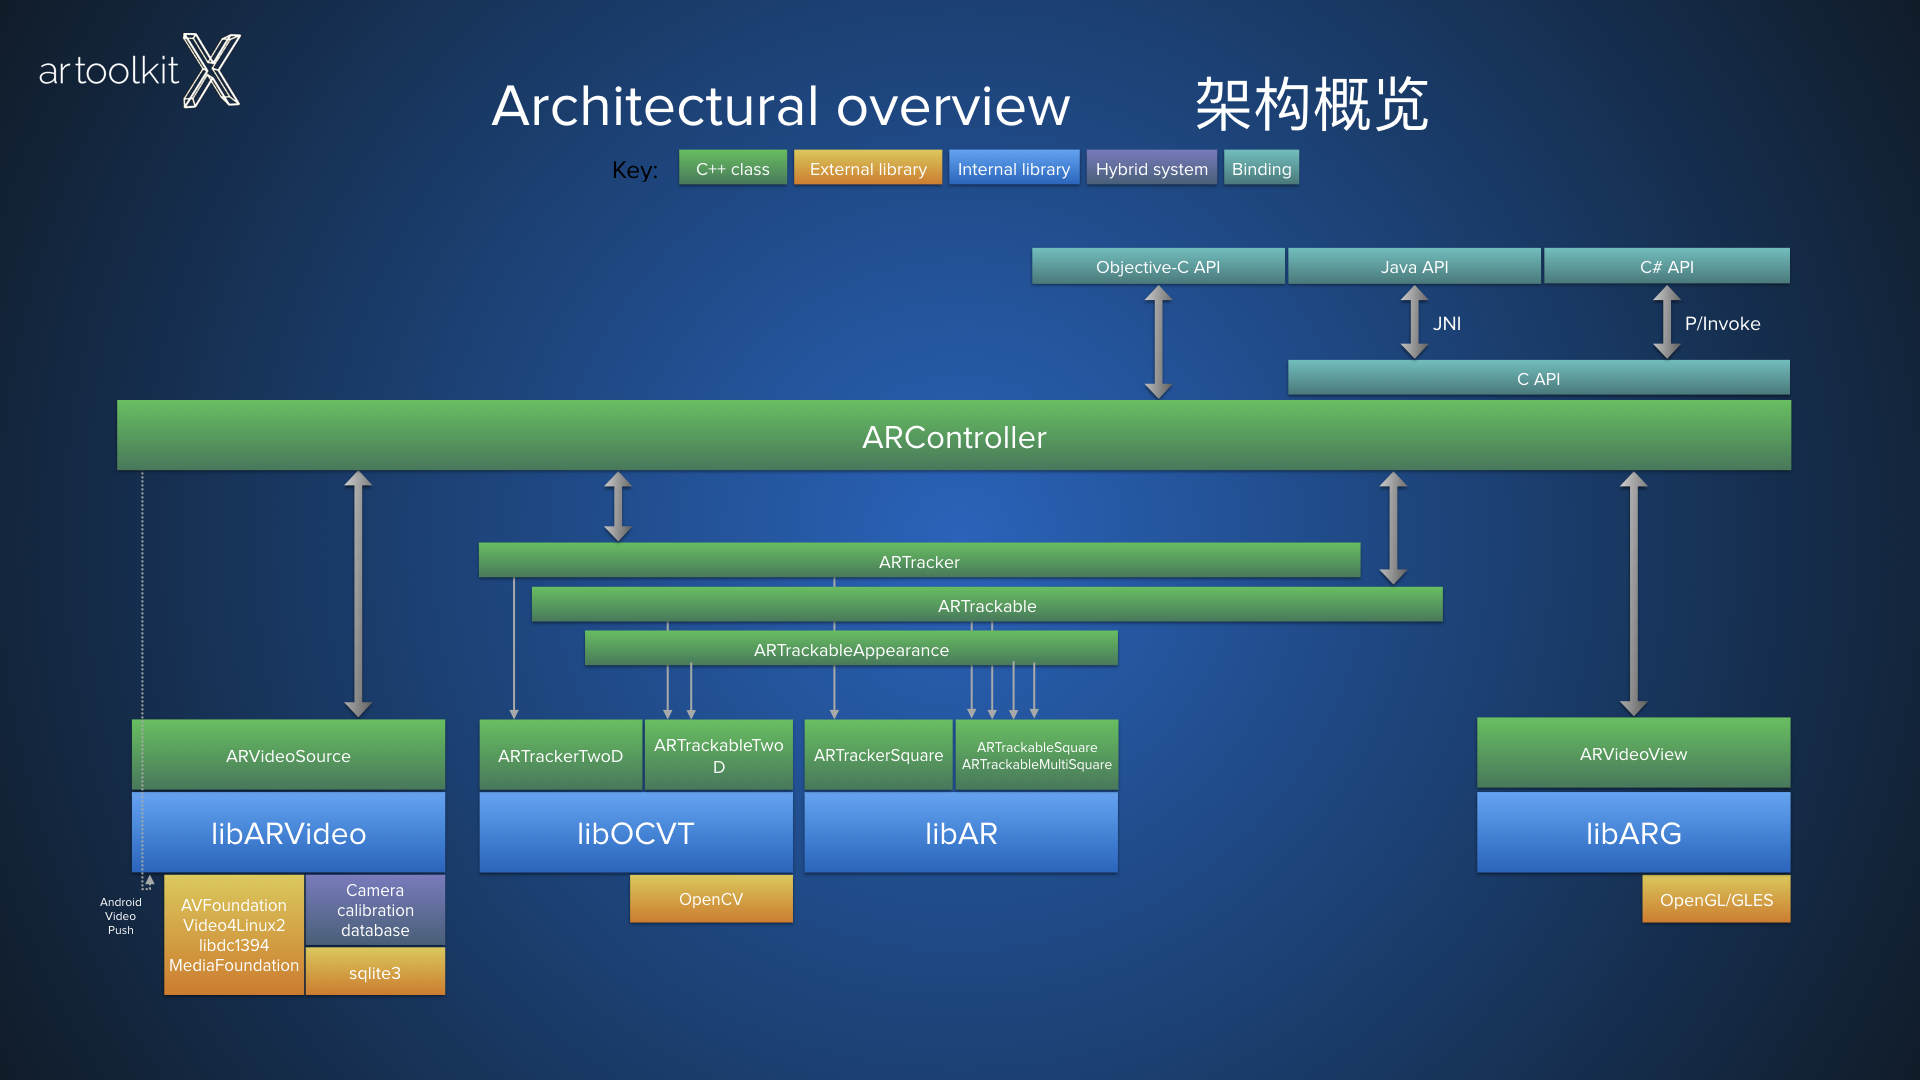
\includegraphics[width=0.8\textwidth]{Abbildungen/artoolkitx-architecture.png}
\caption[ARToolKitX Architektur]{Ein Überblick über die Architektur von ARToolKitX. (Quelle: \cite{artoolkitx:architecture})}
\label{fig:artoolkitx-architecture}
\end{figure}
Grundlegend besteht ARToolKitX aus einer Reihe an C++ Klassen, mit Schnittstellen zu den verschiedenen Programmiersprachen (vergleiche Abbildung \ref{fig:artoolkitx-architecture}).


\section{Beispielhafte Anwendungen}

\subsection{Atlas der Humananatomie}\label{sec:atlas-humananatomie}
Visible Body stellt mit der Anwendung \glqq Atlas der Humananatomie 2020\grqq{} eine Anwendung zur Visualisierung von anatomischen Modellen bereit. \todo{zitieren?} Diese steht auch Studenten der Universität Oldenburg über den Bibliothekszugang zur Verfügung und kommt im medizinischen Bereich zum Einsatz. \\
\subsubsection{Anwendung}
Innerhalb der Applikation stehen dem Nutzer verschiedene anatomische Modelle zur Auswahl. Wird eines dieser Modelle ausgewählt wird es zunächst vor einem eintönigen Hintergrund angezeigt. Allerdings besteht zusätzlich die Möglichkeit das Modell im Augmented Reality Bereich darzustellen (siehe \ref{fig:atlas-skelett)}. \\
Mit Hilfe von Gesten kann der Nutzer mit dem Modell interagieren.
\begin{figure}[h!]
\centering
\includegraphics[width=0.8\textwidth]{Abbildungen/app-atlas-skelett.png}
\caption[Atlas der Humananatomie]{Die Darstellung des menschlichen Skeletts in der Anwendung \glqq Atlas der Humananatomie 2020\grqq . (Quelle: Screenshot aus der Anwendung \glqq Atlas der Humananatomie 2020\grqq )}
\label{fig:atlas-skelett}
\end{figure}

\chapter{Entwicklung}\label{sec:Einleitung}

\section{Anforderungen}\label{Anforderungen}
\section{Konzeptentwurf}\label{Konzeptentwurf}
\section{Implementierung}\label{Implementierung}
\section{Tests}\label{Tests}
\chapter{Evaluation}\label{chapter:evaluation}
In diesem Kapitel werden die Ergebnisse der Arbeit evaluiert. \\
Dabei werden zwei Ziele verfolgt. Zum einen soll der Prototyp anhand der gestellten Anforderungen bewertet werden und zum anderen sollen Probleme und Verbesserungspotentiale des entwickelten Konzepts und der Umsetzung des Prototyps erfasst werden. \\
Dazu wird die Evaluation anhand der Evaluationsziele in eine bewertende Evaluation, bei der die Anwendung auf bestimmte Systemeigenschaften überprüft werden soll, und eine analytische Evaluation, welche die Schwachstellen des Prototyps herausarbeiten soll, unterteilt \citep{hegner:evaluation}.


\section{Bewertende Evaluation}\label{sec:bewertende-evaluation}
Dieses Kapitel dient dazu den Prototypen anhand bestimmter Systemeigenschaften, den in Kapitel \ref{chapter:anforderungsanalyse} gestellten Anforderungen, zu evaluieren. 

\subsection{Vorgehen}
Um den finalen Prototyp auf die gestellten Anforderungen zu überprüfen, wurde dieser auf das Testgerät (ein Huawei P30 Pro) geladen und verschiedenen Testfällen unterzogen, die zum Großteil bereits in Kapitel \ref{sec:tests} beschrieben wurden. Eine genaue Dokumentation von jedem einzelnen Test ist in ..... zu finden. \todo{Verweis auf Testdokumentation}
Im folgenden Abschnitt werden einmal die Ergebnisse des abschließenden Testes zusammengefasst.

\subsection{Ergebnisse}
\subsubsection{Allgemeine Anforderungen}
Insgesamt wurden alle Anforderungen, die sich an die Art der Implementierung richten, umgesetzt.
So läuft die Anwendung auf dem Huawei P30 Pro und wurde dem entsprechend mit Android und Android Studio entwickelt. Auch die Anforderung, dass ein kamera- und markerbasiertes Verfahren verwendet werden soll wurde erfüllt.
\subsubsection{Tracking}
Die Tests haben gezeigt, dass das Tracking stabil mit 60 FPS läuft. Dabei ist es stabil invariant gegenüber verschiedenen Umgebungsveränderungen. Lediglich starke Belichtungswechsel konnten für minimale Aussetzer bei dem Tracking sorgen.

\subsubsection{Modelldarstellung}
Die Modelle, die im OBJ-Format hochgeladen wurden konnten in der Anwendung korrekt mit der richtigen Transformation dargestellt werden und auch die Texturen, die als jpeg oder png-Datei hochgeladen wurden, wurden korrekt angewandt. Bei den Testmodellen wurden sowohl simple selbst erstellte Modelle getestet, als auch sehr komplexe Modelle aus dem Internet mit bis zu 600.000 Faces (Flächen). Alle konnten ohne Problem angezeigt werden, jedoch erhöhen sich die Ladezeiten, je mehr Modelle in die Anwendung geladen wurden und je größer diese sind, dem entsprechend stark. Auch die FPS Anzahl wurde bei vielen gleichzeitig zu rendernden Modellen entsprechend beeinflusst. Diese ist aber erst bei mehreren 100 MB wirklich zu beachten. So sank bei einem Extremtesr die Framerate bei dem parallelen Rendern von drei Modellen mit kombiniert etwa 1.000.000 Faces  (eine DAteigröße von ungefähr 100 MB) und deren Texturdateien, die zusammen ebenfalls eine Größe von fast 100 MB hatten, von den anfänglichen 60 auf 25 FPS. Diese Framerate ist noch nicht bedenklich, da das Tracking zwar weiterhin flüssig war, jedoch sollte diese Auswirkung, besonders mit Blick  auf ältere Geräte, bedacht werden. \\
Da allerdings sein so großer Detailgrad auf einem relativ kleinen Smartphone- oder Tabletdisplay, kaum erkennbar ist, ist eine generelle Vorverarbeitung der Modelle, bei der die Anzahl der Faces(), also der einzelnen Flächen aus denen das Modell besteht, verringert werden, sinnvoll. Dieser Schritt ist sowie so sinnvoll, da die Modelle aus dem Internet oftmals in einer falschen Größe und Rotation vorliegen und kann ohne große Modellierungskenntnisse in kostenlosen Programmen, wie Blender, durchgeführt werden.\\
Als Richtwert, wäre hier ein eine maximale Anzahl von 150.000 Faces und eine maximale Textur Auflösung von 2500x2500 Pixeln denkbar, da ein höherer Detailgrad mit dem bloßen Auge kaum wahrnehmbar. Die Verwendung von speichereffizienten Bildformaten, wie jpeg anstelle von png, ist eine zusätzliche Möglichkeit die Ladezeiten zu verringern.

\subsubsection{Markergenerierung}
Eine weitere Eigenschaft die getestet wurde war die Markergenerierung. Hier erfüllt die Anwendung alle Kriterien und kann insgesamt 4.194.304 Marker generieren. Anhand einer stichprobenartigen Überprüfung (vergleiche Kapitel \ref{sec:test-marker}) konnte festgestellt werden, dass die generierten Marker auch problemlos im Tracking mit der korrekten ID erkannt werden.

\subsubsection{Benutzeroberfäche}
Die Benutzeroberfläche ist simple gehalten und bietet Navigationsmöglichkeiten zu allen wichtigen Funktionen. So sind Ansichten zum Hochladen und Verwalten von Modellen, zur Markergenerierung und zum Tracking vorgesehen. Eine Einschätzung der Usability des User Interfaces wird im nächsten Abschnitt vorgenommen. \\
Ein Problem das der Prototyp noch aufweist ist allerdings, dass die Kameraansicht, sowie die Modelle um 90 Grad gekippt sind.

\section{Analysierende Evaluation}
In einem zweiten Schritt sollten mit Hilfe eines Usability-Tests, bei dem potentielle Nutzer Anwendungsfälle, die sie mit dem Prototyp durchlaufen sollen, vorgelegt bekommen, Fehler und Optimierungsmöglichkeiten gefunden werden. Außerdem sollte die Anwendung im Hinblick auf ihren praktischen Nutzen getestet werden.\\ 
Bei der Erstellung und Durchführung wurde sich an dem in \cite[Kapitel 4]{hegner:evaluation} beschriebenen Verfahren eines Usability-Tests orientiert.

\subsection{Untersuchungsziel}
Das Ziel des Usability-Testes ist es den entwickelten Prototypen dieser Arbeit auf seine Nutzbarkeit zu testen. Dadurch fällt der durchgeführte Test nach \cite[S. 37]{hegner:evaluation} in die Kategorie der bewertenden Tests, die ein neues Produkt vor der weiteren Einführung bewerten sollen.


\subsection{Auswahl der Testnutzer}
Nach \cite[S. 38]{hegner:evaluation} sollte die Stichprobe eine Gruppengröße von 6 bis maximal 20 repräsentativen Nutzern umfassen. \\
Vor der Auswahl der Versuchspersonen, ist es notwendig ein Benutzerprofil zu erstellen, das die Zielgruppe der Anwendung beschreibt. \\
Für den entwickelten Prototypen ist die Hauptzielgruppe, der Bildungsbereich und dabei speziell das höhere Schulniveau und die Universität. Fachlich gesehen eigenen sich vor allem die Naturwissenschaften, mit der Medizin, der Biologie und der Chemie, zum Einsatz der Anwendung. Grundvoraussetzung ist hier das dreidimensionale Modelle Bestandteil des Lerninhaltes sind. Sekundär wäre auch ein Nutzen im Bereich der Geologie oder der Geschichte denkbar. Zu dem richtet sich diser erste Prototyp vor allem an das selbstorganisierte Lernen und somit die älteren Altersstufen, da die Modelle selbst eingefügt werden müssen und nicht direkt von einem Lehrenden innerhalb der Anwendung bereitgestellt werden können. \\
Problematisch bei der Auswahl der Versuchspersonen hat sich die Corona-Pandemie herausgestellt, da die Tests in Präsenz stattfinden mussten.
Dadurch ist zum einen die Größe und Repräsentanz der Stichprobe gesunken.\\
\todo{Beschreibung der gewählten Versuchspersonen}

\subsection{Testaufgaben}
Bei der Wahl der Aufgabe wurde sich an dem Anwendungsfall orientiert das ein Lernender ein Modell an ein Dokument heften möchte. Dazu wurden den Versuchspersonen, die folgenden problemorientierte Aufgabe gegeben:
\glqq Sie haben in Google Drive im Ordner Modelle verschiedenen dreidimensionale Modelle abgelegt. Bitte laden Sie eins dieser Modelle in der Anwendung hoch und speichern Sie den erzeugten Marker in dem Ordner Marker in Google Drive, damit Sie ihn später in ein Dokument einfügen können. Anschließend lassen Sie sich bitte ihr gewähltes Modell auf dem beiliegenden Testdokument, in dem ihr Marker bereits eingefügt worden ist anzeigen. Nun haben Sie die Möglichkeit mit der Darstellung zu experimentieren. \grqq
Damit die Testperson den Marker nicht eigenständig mit Hilfe eines externen Programms in ein Dokument einfügen muss, wird der Person ein solches Dokument bereits beigelegt. Da die Anwendung immer die nächst freie ID verwendet, kann auch bereits der Marker in dieses eingefügt werden.

\subsection{Testumgebung}
Als Testumgebung wurde nach dem Prinzip der Felduntersuchung der Arbeitsplatz also der Schreibtisch der jeweiligen Versuchspersonen gewählt, um die Anwendung in einer realistischen Arbeitsumgebung testen zu können \citep[S. 44]{hegner:evaluation}.

\subsection{Durchführung}
Die Testdurchführung hatte den folgenden Aufbau (nach \cite[S. 46]{hegner:evaluation}):
\begin{enumerate}
\item Begrüßung der Versuchspersonen.
\item Erklärung der Intention des geplanten Tests.
\item Vorlegen der Einverständniserklärung
\item Durchführen des 1. Teils des Interviews
\item Vorstellung des Prototypen und ein grober Überblick über die Funktionen und den Zweck des Prototypen.
\item Erklärung der Aufgabe.
\item Klärung von Fragen.
\item Beginn des Usability-Tests.
\item Durchführen des 2. Teils des Interviews
\item Für Teilnahme bedanken.
\end{enumerate} 

\subsection{Datenerfassung und Dokumentation}
Die Hauptmethode der Datenerfassung stellt ein Interview dar, welches in 2. Teile gegliedert ist. Der erste Teil sollte vor dem Test durchgeführt werden, um das Vorwissen und die Erwartungen zu klären. Der zweite Teil bezog sich dann auf den Usability-Test und wurde dem entsprechend im Anschluss durchgeführt. Inhaltlich sollte im zweiten Teil Probleme und Verbesserungen im Umgang mit dem Prototypen und einem Einsatz von Augmented Reality aufgedeckt werden.\\
Des weiteren wurden während der Benutzer die Aufgaben mit dem Prototypen bewältigt hat, die Beobachtungen notiert, um auftretende Probleme und Abweichungen zum erwarteten Verhalten zu dokumentieren.
\todo{Verweis auf Interviewbogen}

\subsection{Ergebnisse}
Auf Grund der Corona-Pandemie konnte der Utility-Test nur mit einer repräsentativen Versuchsperson durchgeführt werden. \todo{ Verweis dokument} \\
Diese Testperson war aus dem Bereich der (Human-) Medizin und hatte noch keine wirklichen Erfahrungen mit der Augmented Reality im Bildungsbereich gemacht.\\
Generell konnte die Aufgabe ohne wirkliche Probleme bewältigt werden. Jedoch war die Dateistruktur der Modelldateien bestehend aus einer Obj- und einer Texturdatei etwas verwirrend für die Testperson. Im nachfolgenden Interview wurde angemerkt, dass an dieser Stelle eventuell etwas mehr Erklärungen oder ein Info-Button angefügt werden könnte.\\
Auf die Frage, ob der ein Einsatz in der Praxis für die Versuchsperson in Frage kommen würde, wurden die folgenden Einsatzmöglichkeiten erläutert:
\begin{itemize}
\item Die Testperson hält in ihrem Studiengang regelmäßig Vorträge, bei denen Sie sich einen Einsatz der Technologie vorstellen könnte, in dem im Rahmen der Präsentation an den Modellen bestimmte Inhalte gezeigt oder diese im Nachhinein im Rahmen eines Handouts zur Verfügung gestellt werden könnten.
\item Außerdem fasst die Versuchsperson regelmäßig die Vorlesungen zusammen und könnte sich dabei vorstellen die Modelle beziehungsweise Marker in die Zusammenfassungen einzubauen.
\item Eine weitere Möglichkeit, die sich mehr auf den Professor bezieht, wäre es laut der Person, dass der dieser die Modelle in seine Vorlesung einbauen könnte.
\end{itemize}
Besonders hervorgehoben wurde dabei von der Versuchsperson, dass sich die zweite Einsatzmöglichkeit dann eignen würde, wenn die Modelle durch den Professor zur Verfügung gestellt werden würden.\\
Als Verbesserungen und Erweiterungen würde sich die Person noch eine Möglichkeit wünschen, das Modell zu vergrößern. Dieses deckt sich mit dem in der Vision definierten Interaktionsmöglichkeit, die im ersten Prototyp noch nicht umgesetzt wurde (vergleiche Kapitel \ref{sec:vision}).  \\
Des weiteren wurden natürlich auch die in der \nameref{sec:bewertende-evaluation} angesprochen.
Der letzte Punkt der angemerkt wurde war das auch detailreichere Modelle interessant wären, diese Anforderung bezieht sich jedoch nicht auf den Prototypen, sondern viel mehr auf die Modellauswahl.


\chapter{Fazit}\label{chapter:fazit}
Dieses Kapitel zieht ein Fazit über die Ergebnisse und den Verlauf dieser Arbeit. Zudem wird ein Ausblick gegeben.

\section{Zusammenfassung}\label{sec:zusammenfassung}
Augmented Reality stellt eine spannende Möglichkeit zur Verbesserung des Unterrichts dar. Richtig eingesetzt, bietet es die Möglichkeit, nicht nur die Motiavtion, die Ergebnisse und Fähigkeiten der Lernenden zu Verbessern, sondern kann auch die Lehrstrukturen verbessern, in dem es erlaubt, die starren Strukturen eindimensionaler Unterrichtmethoden zu durchbrechen. Es ermöglicht einseitigen Vorträgen der Lehrenden eine interaktive Komponente zu verleihen, durch welche die Lernenden Wissenskonzepte selbst erforschen können.\\
Dabei werden momentan viele spannende Konzepte und Ideen zum Einsatz von Augmented Reality in der Bildung erforscht, deren genauer Mehrwert vermutlich letztendlich weitere Studien und Praxistests benötigt. \\
Im Rahmen dieser Arbeit wurde dann auf Grundlage existierender Arbeiten eine eigenen Augmented Reality Anwendung für den Bildungsbereich entwicklt. In der Art der Wissensvermittlung orientiert sich die Anwendung dabei an Beispielen aus der Praxis wie \glqq Atlas der Humananatomie\grqq . \\
Dabei grenzt sich der entwickelte Prototyp aber durch den Einsatz von Markern und dem Fokus auf eigene Modelle von existierenden Lösungen ab. Durch den Einsatz dieser Marker ist es möglich die Modelle mit anderen Formen der Wissensdarstellung zu verknüpfen. So kann der Marker beispielsweise an Textpassagen angehängt werden, die dem Nutzer weitere Informationen liefern. Dieses ist vor allem dann relevant, wenn man versucht verschiedene Lehrtechniken zu kombinieren. \\
Das Hochladen eigener Modelle ermöglicht zudem eine deutlich bessere Anpassbarkeit an die Anforderungen der Vorlesung und den Endnutzer. Jedoch geht dieses mit der Herausforderung der Beschaffung beziehungsweise Bereitstellung der Modelle einher.\\
Die Evaluation hat dabei gezeigt, dass zum einen die definierten Anforderungen erfüllt werden können und zum anderen konnte mit dem Usability-Test gezeigt werden, dass der Einsatz einer solchen Anwendung in der Praxis durchaus realistisch ist. 

\section{Kritische Reflexion}\label{sec:reflexion}
Insgesamt sind die Ergebnisse der Arbeit als durchaus positiv zu bewerten und auch das Endprodukt, der entwickelten Prototyp, konnte in großen Teilen die Vorstellungen im Vorfeld der Arbeit erfüllen. Ärgerlich ist dabei jedoch, dass die Probleme bezüglich des Portrait-Modus nicht behoben werden konnten. Diese Probleme wurden in der ARToolKitX Beispielanwendung mit Hilfe einer Quick\& Dirty-Lösung behoben, die jedoch aufgrund der Neuerungen, wie der Navigation, im Prototypen nicht mehr genutzt werden konnte. Vor allem an dieser Stelle hat sich die mangelnde Dokumentation von ARToolKitX bemerkbar gemacht. Diese Tatsache zusammen mit dem Problem, das ebenfalls kaum Forumeinträge zu ARToolKit spezifischen Problemen existieren, hat extrem viel Zeit in Anspruch genommen. \\
So bestand ein Großteil allein darin die Strukturen von ARToolKitX zu verstehen, indem der Programmcode der Klassen durchgearbeitet wurde.\\
Ein weiterer Punkt der leider nicht wie gewünscht umgesetzt werden konnte bezog sich auf die Evaluation. Hier mussten die Tests mit dem Nutzer aufgrund der Kontaktbeschränkungen in einem deutlich geringeren Rahmen durchgeführt werden. Geplant war es an dieser Stelle eigentlich mit verschiedenen Nutzergruppen, wie Professoren, Tutoren und Studenten aus verschiedenen Fachbereichen zu testen. Dieses konnte leider nicht umgesetzt werden.\\
Betrachtet man Rückblickend den gesamten Verlauf der Arbeit, ist der Start durch aus kritisch zu betrachten. Dort fehlte es an einem konkreten Startdatum, wodurch es nie wirklich den Punkt gab, ab dem mit Blick auf ein konkretes Ende hingearbeitet wurde. Ein Punkt der vermutlich dazu beigetragen hat, ist das die Arbeit zu Beginn der Corona-Pandemie begonnen wurde und die ganzen internen Abläufe der Universität Oldenburg überarbeitet werden mussten.\\

\section{Ausblick}\label{sec:ausblick}
Der entwickelte Prototyp stellt nur eine erste Version der in der \nameref{chapter:anforderungsanalyse} definierten Vision dar, welche noch in vielen Bereichen erweitert werden kann. \\
Ein Punkt der auch in dem Usability-Test wiederfindet ist die Erweiterung um eine Interaktionsmöglichkeit. Hier könnte mit Hilfe von Gestend das Modell vergrößert oder gedreht werden. \\
Der nächste große Schritt wäre es dann den Nutzern die Möglichkeit zugeben die Modelle mit anderen Nutzern zu teilen. Dazu könnte Beispielsweise das in der \nameref{sec:vision} definierte Konzept mit einem Raumcode umgesetzt werden. Diese Eigenschaft ist auch essentiell, um das Anwendungsszenario, bei dem der Professor die Modelle und Marker in seine Vorlesung einbaut umzusetzen. Dieses wurde sowohl zu Beginn bei der \nameref{chapter:anforderungsanalyse} definiert als auch bei der Nutzer-Evaluation herausgearbeitet. \\
Neben den konkreten Umsetzungen ist auch ein weiteres Erforschen der speziellen Anforderungen des Bildungsbereiches sinnvoll. Der Prototyp stellt eine erste Grundlage dar, für den in einem nächsten Schritt die Anforderungen und der konkrete Anwendungsfall verfeinert werden sollte. Dazu wären unter anderem eine konkrete Anforderungserhebung in der Praxis und mit Lehr- und Fachkräften denkbar. 

\chapter{Beispielkapitel}\label{sec:beispiel}

Hier etwas Text mit einer Notiz.\todo{Vergiss mich nicht!}

\section{Abschnitt}\label{test:test2}

Möchste man eine Referenz z.B. am Ende eines Satzes oder Absatzes setzen, dann mit Klammern: \citep[S. 5]{hevner04:design}

Möchte man die Autoren als Substantiv direkt im Satz verwenden, dann ohne Klammern: \citet{hevner04:design}

Nur Autoren: \citeauthor{hevner04:design}

Nur Jahr der Veröffentlichung: \citeyear{hevner04:design}

Beispiel für eine Webquelle: \cite{internet00:webquelle}

Referenz auf dieses Kapitel mit seinem Namen: \nameref{sec:beispiel}

Referenz auf dieses Kapitel mit seiner Bezeichnung und Nummer: \autoref{sec:beispiel}

Referenz auf dieses Kapitel nur mit seiner Nummer: \ref{sec:beispiel}

\subsection{Unterabschnitt}

\begin{figure}[h!] %Für längere Arbeiten ist [h!] zur Positionierung meist in Ordnung
\centering

\includegraphics[width=0.4\textwidth]{Abbildungen/uni_ol_logo.png}
\caption[Name der Abbildung im Tabellenverzeichnis]{Beschreibung der Abbildung}
\label{fig:figure}
\end{figure}

\subsubsection{Unterunterabschnitt}

\begin{table}[h!] %Für längere Arbeiten ist [h!] zur Positionierung meist in Ordnung
\centering
\begin{tabular}{|c|c|}
\hline 
1 & 2 \\ 
\hline 
a & b \\ 
\hline 
\end{tabular} 
\caption[Name der Tabelle im Tabellenverzeichnis]{Beschreibung der Tabelle}
\label{tab:tabelle}
\end{table}

\section{Ipsum}
Lorem ipsum dolor sit amet, consetetur sadipscing elitr, sed diam nonumy eirmod tempor invidunt ut labore et dolore magna aliquyam erat, sed diam voluptua. At vero eos et accusam et justo duo dolores et ea rebum. Stet clita kasd gubergren, no sea takimata sanctus est Lorem ipsum dolor sit amet. Lorem ipsum dolor sit amet, consetetur sadipscing elitr, sed diam nonumy eirmod tempor invidunt ut labore et dolore magna aliquyam erat, sed diam voluptua. At vero eos et accusam et justo duo dolores et ea rebum. Stet clita kasd gubergren, no sea takimata sanctus est Lorem ipsum dolor sit amet. Lorem ipsum dolor sit amet, consetetur sadipscing elitr, sed diam nonumy eirmod tempor invidunt ut labore et dolore magna aliquyam erat, sed diam voluptua. At vero eos et accusam et justo duo dolores et ea rebum. Stet clita kasd gubergren, no sea takimata sanctus est Lorem ipsum dolor sit amet.   

Duis autem vel eum iriure dolor in hendrerit in vulputate velit esse molestie consequat, vel illum dolore eu feugiat nulla facilisis at vero eros et accumsan et iusto odio dignissim qui blandit praesent luptatum zzril delenit augue duis dolore te feugait nulla facilisi. Lorem ipsum dolor sit amet, consectetuer adipiscing elit, sed diam nonummy nibh euismod tincidunt ut laoreet dolore magna aliquam erat volutpat.   

Ut wisi enim ad minim veniam, quis nostrud exerci tation ullamcorper suscipit lobortis nisl ut aliquip ex ea commodo consequat. Duis autem vel eum iriure dolor in hendrerit in vulputate velit esse molestie consequat, vel illum dolore eu feugiat nulla facilisis at vero eros et accumsan et iusto odio dignissim qui blandit praesent luptatum zzril delenit augue duis dolore te feugait nulla facilisi.  
%--------------------------
%---Literaturverzeichnis---
%--------------------------

%Dokument vollständig setzen:
%latex
%bibtex
%latex
%latex

\cleardoublepage
\phantomsection
\addcontentsline{toc}{chapter}{Literaturverzeichnis} %Literaturverzeichnis im Inhaltsverzeichnis aufführen

\bibliography{Bibliographie/Bibliographie} %Bibliographie-Datei ohne .bib-Endung angeben!

%------------
%---Anhang---
%------------

\appendix %nummerierte Kapitel im Anhang mit Buchstaben statt Zahlen

\chapter{Beispielanhang}

Beispiel für einen Anhang! %auskommentieren, falls nicht benötigt

%-------------
%---Schluss---
%-------------

\backmatter %Keine nummerierten Kapitel für z.B. Glossar, Index, Erklärung, etc.

\pagenumbering{gobble} %keine Seitenzahl auf der Erklärung
\chapter*{Erklärung}
Hiermit versichere ich, \autor{}, dass ich diese Arbeit selbständig verfasst und keine anderen als die angegebenen Quellen und Hilfsmittel benutzt habe. Außerdem versichere ich, dass ich die allgemeinen Prinzipien wissenschaftlicher Arbeit und Veröffentlichung, wie sie in den Leitlinien guter wissenschaftlicher Praxis der \universitaet{} festgelegt sind, befolgt habe.

\vspace{3cm}

{\def\arraystretch{2}
\begin{tabular}{p{8cm}}
\hline 
\autor \\ 
\end{tabular}
}

 %Erklärung auf der letzten Seite der gesamten Arbeit



\end{document}